\documentclass{article}
\usepackage{graphicx}% Required for inserting images
\usepackage{lindrew}
\usepackage[shortlabels]{enumitem}
\usepackage{enumerate}
\usepackage{algorithm}
\usepackage{algpseudocode}
\usepackage{matlab-prettifier}
\usepackage{pythonhighlight}

\title{CS 156a Problem Set 5}
\author{Amitesh Anand Pandey}
\date{October 2024}

\begin{document}
\maketitle
\section*{Linear Regression Error}
\subsection*{Problem 1}
We know that 
\begin{equation*}
    \mathbb{E}_{\mathcal{D}}[E_{\text{in}}(\mathbf{w}_{\text{lin}})] = \sigma^{2}\left(1 - \frac{d+1}{N}\right)
\end{equation*}
Letting $\mathbb{E}_{\mathcal{D}}[E_{\text{in}}(\mathbf{w}_{\text{lin}})] = 0.008, d=8, \sigma = 0.1$, we have
\begin{equation*}
    0.008 = 0.01\left(1 - \frac{9}{N}\right) \implies 1 - \frac{0.008}{0.01} = \frac{9}{N} \implies N = \frac{9}{1 - \frac{0.008}{0.01}} \implies N = 45
\end{equation*}
so among the choices $N = 100$, $\textbf{[c]}$ is the correct option.
\section*{Nonlinear Transforms}
\subsection*{Problem 2}
We need $\text{sign}(\Tilde{\mathbf{w}}^{T}\cdot(1,x_{1}^{2},x_{2}^{2}))$ to be negative for extreme $x_1$ and positive only for non-extreme $x_2$. We have
\begin{equation*}
    \Tilde{w}_0 + \Tilde{w}_{1}x_{1}^{2} + \Tilde{w}_{2}x_{2}^{2}
\end{equation*}
For large $x_{1}$, the square will be even larger, thus $\Tilde{w}_{1}$ would have to make it negative by being $\Tilde{w}_{1} < 0$. Now notice that for most of large $x_{2}$, we have the point classified as positive. Thus $\Tilde{w}_{2} > 0$ to bring the overall sum towards the positive side. Thus $\textbf{[d]}$, $\Tilde{w}_{1} < 0$ and $\Tilde{w}_{2} > 0$ is correct.
\subsection*{Problem 3}
The $d_{\text{VC}} \leq d_{\mathbf{\Phi}}  +1$, and $d_{\mathbf{\Phi}} = 14$, so $d_{\text{VC}} \leq 15$. This means $\textbf{[c]}$ is the correct option.
\newpage
\section*{Gradient Descent}
\subsection*{Problem 4}
The partial derivative
\begin{equation*}
    \frac{\partial E}{\partial u} = 2(ue^{v} - 2ve^{-u})\frac{\partial}{\partial u}(ue^{v} - 2ve^{-u}) = 2(ue^{v} - 2ve^{-u})(e^{v} + 2ve^{-u})
\end{equation*}
employing chain rule for partial derivatives. Thus $\textbf{[e]}$ is the correct option.
\subsection*{Problem 5}
From using this \hyperref[prob5]{code}, we get the iterations as 10, so $\textbf{[d]}$ is the correct option.
\subsection*{Problem 6}
Once again, using this \hyperref[prob5]{code}, we find that the point $(0.045, 0.024)$ is closest to our values of $u,v$ at the 10th iteration, which means that $\textbf{[e]}$ is the correct option. 
\subsection*{Problem 7}
Essentially, instead of simultaneously affecting a change in $u, v$, we're doing it stepwise, first with $u$, then with $v$. See the \hyperref[prob6]{code}, we have that $\textbf{[a]}$, $\text{Error} = 0.1$ is the closest to ours, $0.139$. 
\section*{Logistic Regression}
\subsection*{Problem 8}
Figure 1 is an image of a 100 random points in $[-1, 1]\times[-1,1]$ classified through a randomly generated line (target), for visualization purposes.
\begin{figure}[htp]
    \centering
    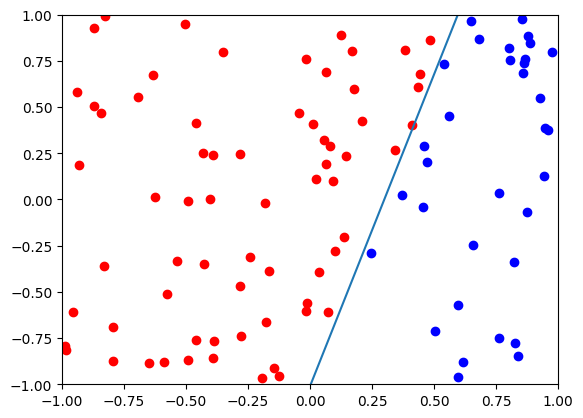
\includegraphics[width=2in]{plothw5.png}
    \caption{100 randomly uniformly picked points classified with a random target}
    \label{fig:galaxy}
\end{figure}
For $N = 100$, using this \hyperref[prob8]{code}, the average $E_{out} \approx 0.1$, thus $\textbf{[d]}$ is correct.
\subsection*{Problem 9}
Using \hyperref[prob8]{code}, we find that average epochs to be $\approx 339$, so $\textbf{[a]}$ is correct.
\newpage
\begin{codexpl*}[Problems 8 and 9]
1. \verb|generate_target|: Generates two random points in $[-1,1]\times [-1,1]$, and creates a line between them as the boundary for classification. Obtains intercept by plugging calculated slope back into one of the points.\\
2. \verb|classify_point|: Takes a point in $[-1,1]\times[-1,1]$ and labels it as $+1$ if it falls under the target line and $-1$ otherwise. \\
3. \verb|generate_dataset|: Takes the desired size of dataset and a target function on the basis of which, it not only generates the desired number of points but also labels them, thereby creating a total dataset of randomly picked points along with their labels. \\
4. \verb|gradient|: Takes labelled point generated in the format of \verb|generate_dataset[i]| and weight vector, and applies one iteration/step of stochastic gradient descent on this point, thereby returning the values necessary for updating the weight vector later on. 
\end{codexpl*}
\section*{PLA vs SGD}
\subsection*{Problem 10}
Recall that the PLA can be expressed as having $1$ when the sign of $w^{T}x$ is positive and $0$ when it's negative. We simply make this change to accommodate the already studied PLA into the paradigm followed in the options. Then, it becomes clear that the SGD error function would be 
\begin{equation*}
    e_{n}(\mathbf{w}) = -\text{min}(0, y_{n}\mathbf{w}^{T}x_{n})
\end{equation*}
Thus $\textbf{[e]}$ is the correct option. 
\newpage
\section*{Appendix}

\subsection{\label{prob5}Gradient Descent Max Error $10^{-14}$}
\begin{lstlisting}[frame=single,
numbers=left,
style=Matlab-Pyglike]
import math

def E(u ,v):
    return (u*math.exp(v) - 2*v*(math.exp(-u)))**2

def dEdu(u,v):
    return ((2)*(math.exp(v) + 2*v*math.exp(-u))*(u*math.exp(v) -2*v*math.exp(-u)))

def dEdv(u,v):
    return ((2)*(u*math.exp(v) -2*v*math.exp(-u))*(u*math.exp(v) - 2*math.exp(-u)))


def gradient_descent(u, v, desired_error, gamma):
    iterations = 0
    cur_error = E(u,v)
    while cur_error > desired_error:
        du = dEdu(u,v)
        dv = dEdv(u,v)
        u = u - gamma*du
        v = v - gamma*dv
        cur_error = E(u, v)
        iterations += 1
    else:
        return (u, v, iterations)

u, v, i = gradient_descent(1,1,10**(-14), 0.1)
print(i)
print('a: ', math.dist([u,v], [1.000, 1.000]))
print('b: ', math.dist([u,v], [0.713, 0.045]))
print('c: ', math.dist([u,v], [0.016, 0.112]))
print('d: ', math.dist([u,v], [-0.083, 0.029]))
print('e: ', math.dist([u,v], [0.045, 0.024]))
\end{lstlisting}
\newpage
\subsection{\label{prob6} Coordinate Descent for 15 iterations}
\begin{lstlisting}[frame=single,
numbers=left,
style=Matlab-Pyglike]
def coordinate_descent(u, v, max_iter, gamma):
    iterations = 0
    cur_error = E(u,v)
    while max_iter > iterations:
        du = dEdu(u,v)
        u = u - gamma*du
        dv = dEdv(u,v)
        v = v - gamma*dv
        cur_error = E(u, v)
        iterations += 1
    else:
        return (cur_error)

error = coordinate_descent(1,1,15, 0.1)
print(error)
\end{lstlisting}
\newpage
\subsection{\label{prob5}Gradient Descent Max Error $10^{-14}$}
\begin{lstlisting}[frame=single,
numbers=left,
style=Matlab-Pyglike]
import math

def E(u ,v):
    return (u*math.exp(v) - 2*v*(math.exp(-u)))**2

def dEdu(u,v):
    return ((2)*(math.exp(v) + 2*v*math.exp(-u))*(u*math.exp(v) -2*v*math.exp(-u)))

def dEdv(u,v):
    return ((2)*(u*math.exp(v) -2*v*math.exp(-u))*(u*math.exp(v) - 2*math.exp(-u)))


def gradient_descent(u, v, desired_error, gamma):
    iterations = 0
    cur_error = E(u,v)
    while cur_error > desired_error:
        du = dEdu(u,v)
        dv = dEdv(u,v)
        u = u - gamma*du
        v = v - gamma*dv
        cur_error = E(u, v)
        iterations += 1
    else:
        return (u, v, iterations)

u, v, i = gradient_descent(1,1,10**(-14), 0.1)
print(i)
print('a: ', math.dist([u,v], [1.000, 1.000]))
print('b: ', math.dist([u,v], [0.713, 0.045]))
print('c: ', math.dist([u,v], [0.016, 0.112]))
print('d: ', math.dist([u,v], [-0.083, 0.029]))
print('e: ', math.dist([u,v], [0.045, 0.024]))
\end{lstlisting}
\newpage
\subsection{\label{prob8} Epochs and Eout for Logistic Regression with SGD}
\begin{lstlisting}[frame=single,
numbers=left,
style=Matlab-Pyglike]
import numpy as np
import random as rand

def generate_target():
    p1 = [random.uniform(-1,1), random.uniform(-1,1)]
    p2 = [random.uniform(-1,1), random.uniform(-1,1)]
    m = (p2[1] - p1[1])/(p2[0] - p1[0])
    b = p2[1] - m*p2[0]
    return [m,b]

N = 100
def classify_point(point, target):
    if target[0]*point[0] + target[1] < point[1]:
        return '+1'
    else:
        return '-1'
    
def generate_dataset(N, target):
    dataset = []
    for i in range(N):
        point = [random.uniform(-1,1), random.uniform(-1,1)]
        y = classify_point(point, target)
        point.append(y)
        dataset.append(point)
    return dataset

f = generate_target()
dataset = generate_dataset(N, f)
xred = []
yred = []
xblue = []
yblue = []
for p in dataset:
    if p[2][0] == '+':
        xred.append(p[0])
        yred.append(p[1])
    else:
        xblue.append(p[0])
        yblue.append(p[1])

from matplotlib import pyplot as plt
plt.scatter(xred,yred,color='red')
plt.scatter(xblue,yblue,color='blue')
plt.axline((-1, -f[0] + f[1]), (1, f[0] + f[1]))
plt.ylim(-1, 1)
plt.xlim(-1, 1)

plt.show()
def gradient(p, w):
    x = [1, p[0], p[1], int(p[2])]
    sum_e = [0, 0, 0]
    
    temp_sum = [x[3] * x[0], x[3] * x[1], x[3] * x[2]]
    for t in range(3):
        temp_sum[t] /= -1 * (1 + math.exp(-1 * (x[3] * (x[0] * w[0] + x[1] * w[1] + x[2] * w[2]))))
        sum_e[t] += temp_sum[t]

    return sum_e


epoch = 0
e_count = 0
gamma = 0.01
num_experiments = 100
num_test_points = 500
for i in range(num_experiments):
    f = generate_target()
    dataset = generate_dataset(N, f)
    
    w = [0, 0, 0]
    wb = [10, 10, 10]
    
    while(math.sqrt((wb[0] - w[0])**2 + (wb[1] - w[1])**2 + (wb[2]-w[2])**2) > 0.01):
        wb = w[:]
        random.shuffle(dataset)
        for j in range(N):
            e_in_sample = gradient(dataset[j], w)
            for k in range(3):
                e_in_sample[k] *= gamma
                w[k] += e_in_sample[k]
        epoch += 1
    
    dataset_error = generate_dataset(num_test_points, f)
    misclassified = 0
    
    for point_idx in range(num_test_points):
        misclassified += math.log(1 + math.exp(int(dataset_error[point_idx][2]) *  
                        (w[0] + w[1] * dataset_error[point_idx][0] + w[2] * dataset_error[point_idx][1])))
    
    e_count += misclassified/num_test_points
    
print("E_out average: " + str(e_count/num_experiments))
print("Epochs taken average: " + str(epoch/num_experiments))
\end{lstlisting}
\end{document}
